\documentclass{standalone}
\usepackage{tikz}
\usetikzlibrary{positioning, decorations.pathreplacing}

\begin{document}
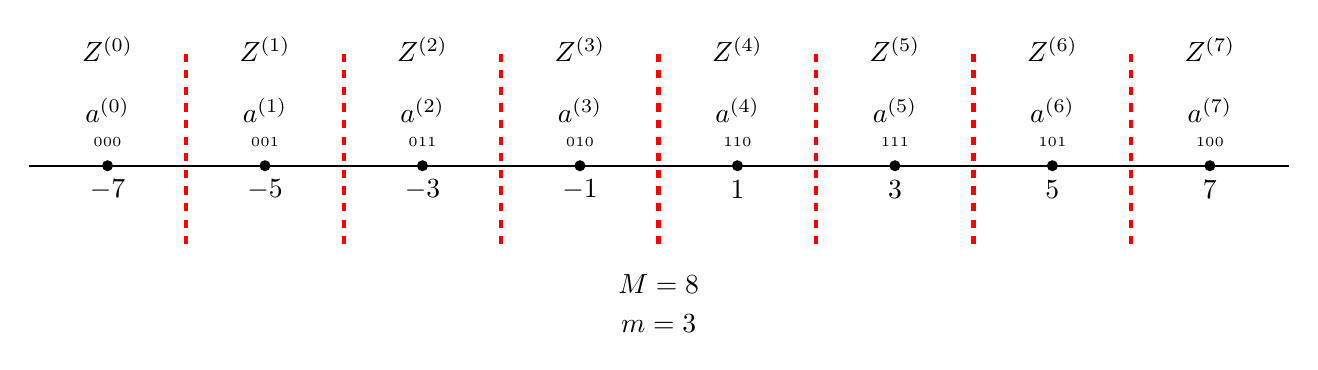
\begin{tikzpicture}

% Define colors
\definecolor{myred}{RGB}{255, 0, 0}

% Draw the horizontal line
\draw[thick] (-8, 1) -- (8, 1);

% Draw the nodes
\fill (-7, 1) circle (2pt);
\fill (-5, 1) circle (2pt);
\fill (-3, 1) circle (2pt);
\fill (-1, 1) circle (2pt);
\fill (1, 1) circle (2pt);
\fill (3, 1) circle (2pt);
\fill (5, 1) circle (2pt);
\fill (7, 1) circle (2pt);

% Add labels for a
\node at (-7, 0.7) {$-7$};
\node at (-5, 0.7) {$-5$};
\node at (-3, 0.7) {$-3$};
\node at (-1, 0.7) {$-1$};
\node at (1, 0.7) {$1$};
\node at (3, 0.7) {$3$};
\node at (5, 0.7) {$5$};
\node at (7, 0.7) {$7$};

% Add binary labels for a
\node at (-7, 1.3) {\textnormal{\tiny $000$}};
\node at (-5, 1.3) {\textnormal{\tiny $001$}};
\node at (-3, 1.3) {\textnormal{\tiny $011$}};
\node at (-1, 1.3) {\textnormal{\tiny $010$}};
\node at (1, 1.3) {\textnormal{\tiny $110$}};
\node at (3, 1.3) {\textnormal{\tiny $111$}};
\node at (5, 1.3) {\textnormal{\tiny $101$}};
\node at (7, 1.3) {\textnormal{\tiny $100$}};

% Add labels for a^(i)
\node at (-7, 1.7) {$a^{(0)}$};
\node at (-5, 1.7) {$a^{(1)}$};
\node at (-3, 1.7) {$a^{(2)}$};
\node at (-1, 1.7) {$a^{(3)}$};
\node at (1, 1.7) {$a^{(4)}$};
\node at (3, 1.7) {$a^{(5)}$};
\node at (5, 1.7) {$a^{(6)}$};
\node at (7, 1.7) {$a^{(7)}$};

% Draw the dashed lines in green
\draw[myred, ultra thick, dashed] (-6, 0) -- (-6, 2.5);
\draw[myred, ultra thick, dashed] (-4, 0) -- (-4, 2.5);
\draw[myred, ultra thick, dashed] (-2, 0) -- (-2, 2.5);
\draw[myred, ultra thick, dashed] (0, 0) -- (0, 2.5);
\draw[myred, ultra thick, dashed] (2, 0) -- (2, 2.5);
\draw[myred, ultra thick, dashed] (4, 0) -- (4, 2.5);
\draw[myred, ultra thick, dashed] (6, 0) -- (6, 2.5);

% Add labels for Z
\node[above] at (-7, 2.2) {$Z^{(0)}$};
\node[above] at (-5, 2.2) {$Z^{(1)}$};
\node[above] at (-3, 2.2) {$Z^{(2)}$};
\node[above] at (-1, 2.2) {$Z^{(3)}$};
\node[above] at (1, 2.2) {$Z^{(4)}$};
\node[above] at (3, 2.2) {$Z^{(5)}$};
\node[above] at (5, 2.2) {$Z^{(6)}$};
\node[above] at (7, 2.2) {$Z^{(7)}$};

% Add the bottom text
\node at (0, -0.5) {$M=8$};
\node at (0, -1) {$m=3$};

\end{tikzpicture}
\end{document}


